\renewcommand{\myauthor}{Christoph Schwaninger}
\subsection{Bauteilauswahl}

\subsubsection{Computer}

Für die Diplomarbeit wurden mehrere Rechner in betracht gezogen, jedoch wurde die Entscheidung zwischen den folgenden beiden getroffen aus dem Grund, dass beide sofort zur Verfügung standen:
\begin{itemize}
\item \textbf{Raspberry Pi 5:} Der Raspberry pi 5 verfügt über einen Quad-Core ARM Cortex-A76 Prozessor wodurch genug Rechenleistung bereitgestellt ist. Zusätzlich bietet dieser genug Schnittstellen um mit einer einfach 8x8 Matrix die Schaltung zu entwickeln. Ein weiterer Punkt ist die gute Dokumentation, möglichen Librarys und die Programmiermöglichkeit mittels Pyhton welche, für Diplomant Maximilian Koch, bevorzugt ist.
Die Nachteile des Raspberry Pi sind zum einen den bnötigten Platz welchen dieser benötigt, die Anschaffungskosten für einen und der höhere Stromverbrauch.\\

\item \textbf{ESP32-S3:} Der ESP32-S3 verfügt über einen Dual-Core-Xtensa-LX7 Prozsessor welcher für das auslesen der Matrix genug Rechenleistung bereitstellen könnte. Für den ESP32-S3 spricht auch seine kompakte Größe, seine geringe Leisutngsaufnahme und die geringen Anschaffungskosten.
Die Nachteile des ESP32 sind zum einen aber auch die begrenzte Rechenleistung. Die weitere Hardware welche auch vom ESP gesteuert wreden muss, könnte den ESP schnell an seine Grenzen bringen und das fehlen eines vollwertigem Betriebssystem welches das Umsetzen von komplexeren Softwarestrukturen erschwert. 
\end {itemize}

Die Entscheidung fiel auf den Raspberry Pi 5, da dieser bereits verfügbar war und über ausreichende Rechenleistung  für das Projekt verfügt. Zudem stellte die Möglichkeit der Programmierung in Python, welche von Diplomant Maximilian Koch bevorzugt wird, einen weiteren ausschlaggebenden Faktor dar, wobei grundsätzlich auch andere Raspberry Pi Modelle für dieses Projekt geeignet gewesen wären.


\subsubsection{Sensoren}

Bei der Auswahl der Sensoren, die zur Erkennung der Spielfiguren sind, wurden mehrere Optionen in betracht gezogen:

\begin{itemize}
\item \textbf{Hall-Sensoren:} 
\begin{table}[H]
\centering
\renewcommand{\arraystretch}{1.3}
\begin{tabular}{|p{4cm}|p{7cm}|}
\hline
\textbf{Merkmal} & \textbf{Beschreibung} \\
\hline
Technologie & Digitaler Hall-Effekt-Sensor \\
\hline
Beispielbauteil & A3144 (Digitaler Sensor) \\
\hline
Betriebsspannung & 4,5 V – 24 V  QUELLE!!!\\
\hline
Ausgang & Digital (Open-Collector) \\
\hline
Funktionsprinzip & Erkennung eines Magnetfeldes durch Hall-Effekt \\
\hline
Vorteile & Kontaktlos, verschleißfrei, hohe Lebensdauer, unempfindlich gegen Staub und Licht \\
\hline
Nachteile & Magnet in jeder Figur erforderlich \\
\hline
Kostenbewertung & Gering \\
\hline
Zuverlässigkeit & Sehr hoch, geringe Fehleranfälligkeit \\
\hline
Praktikabilität & Sehr hoch, klein, einfache Beschaltung \\
\hline
\end{tabular}
\caption{Bewertung der Hall-Sensoren zur Figurenerkennung}
\label{tab:hall}
\end{table}

\item \textbf{NFC/RFID:} 

\begin{table}[H]
\centering
\renewcommand{\arraystretch}{1.3}
\begin{tabular}{|p{4cm}|p{7cm}|}
\hline
\textbf{Merkmal} & \textbf{Beschreibung} \\
\hline
Technologie & NFC / HF-RFID \\
\hline
Beispielbauteile & PN532 oder MFRC522 (Reader), NTAG213 (Tag) \\
\hline
Betriebsspannung & Typ. 3{,}3\,V – 5\,V (modulabhängig) \\
\hline
Ausgang / Schnittstelle & I\textsuperscript{2}C / SPI / UART \\
\hline
Funktionsprinzip & Kontaktlose Identifikation einer Figur über eindeutige Tag-ID \\
\hline
Vorteile & Eindeutige Figurenidentifikation möglich, kontaktlos \\
\hline
Nachteile & Höherer Hardware- und Softwareaufwand, Metalle können Reader beeinflussen \\
\hline
Kostenbewertung & Mittel bis hoch \\
\hline
Zuverlässigkeit & Sehr hoch  \\
\hline
Praktikabilität & Mittel; Integration auf 64 Feldern erfordert Multiplexing \\
\hline
\end{tabular}
\caption{Bewertung von NFC/RFID zur Figurenerkennung}
\label{tab:nfc}
\end{table}
\newpage
\item \textbf{Optische Sensoren:} 

\begin{table}[H]
\centering
\renewcommand{\arraystretch}{1.3}
\begin{tabular}{|p{4cm}|p{7cm}|}
\hline
\textbf{Merkmal} & \textbf{Beschreibung} \\
\hline
Technologie & Infrarot-Reflexionssensor \\
\hline
Beispielbauteile & TCRT5000 oder CNY70 \\
\hline
Betriebsspannung & Typ. 5\,V \\
\hline
Ausgang / Schnittstelle & Analog oder digital (je nach Beschaltung) \\
\hline
Funktionsprinzip & IR-LED sendet Licht; Phototransistor misst reflektiertes Signal \\
\hline
Vorteile & Keine Magnete oder Tags erforderlich, direkte Objekterkennung \\
\hline
Nachteile & Empfindlich gegenüber Fremdlicht und Verschmutzung \\
\hline
Kostenbewertung & Mittel \\
\hline
Zuverlässigkeit & Mittel; abhängig von Lichtverhältnissen, Oberflächenbeschaffenheit und Kalibrierung. \\
\hline
Praktikabilität & Mittel; exakte Ausrichtung und ggf. Kalibrierung pro Feld erforderlich. \\
\hline
\end{tabular}
\caption{Bewertung optischer Sensoren zur Figurenerkennung}
\label{tab:optisch}
\end{table}
\end {itemize}

Nach dem Vergleich der untersuchten Sensortechnologien wurde der digitale Hall-Sensor als bevorzugte Lösung ausgewählt. 
Er bietet eine sehr hohe Zuverlässigkeit durch kontaktlose und verschleißfreie Arbeitsweise bei gleichzeitig geringem Kosten- 
und Integrationsaufwand. 

Optische Sensoren weisen eine erhöhte Empfindlichkeit gegenüber Umgebungslicht, Verschmutzung und Kalibrierungsabweichungen auf, 
wodurch die Langzeitstabilität beeinträchtigt werden kann. NFC/RFID-Systeme ermöglichen zwar eine eindeutige Identifikation 
jeder Figur, verursachen jedoch einen deutlich höheren Hardwareaufwand, insbesondere bei der Umsetzung 
auf 64 Spielfeldern.

Unter Berücksichtigung der Anforderungen an Kosten, Zuverlässigkeit, Integrationsaufwand und Systemkomplexität 
stellt der Hall-Sensor die technisch und wirtschaftlich sinnvollste Lösung für das elektronische Schachbrett dar.

\subsection{Schaltungsentwicklung}

Bei der Entwicklung der Verschaltungslogik muss damit begonnen werden, wie ein einzelner Sensor korrekt ohne Fehler ausgelesen werden kann. Wichtig ist auch, dass der Raspberry pi mit einem Logikpegel von 3,3V arbeitet und die Hall-Sensoren laut Datenblatt eine Spannung von mindestens 4,5V benötigen. Falls die Sensoren nicht mit 3,3V Versorgungsspannung funktionieren muss hier ein Logic-Level-Shifter verwedent werden

Beschaltung des A3144:

Der Hall-Sensor verfügt über jeweils einen VCC, GND und OUT pin.
Der Sensor schaltet den Ausgang nur dann auf LOW, (Open-Collector) wenn der Südpol von einem Magneten in Reichweite ist. 

Die Ausgänge vom Sensor und Verschaltung dieser sehen wie folgt aus:

\begin{figure}[H]
	\centering
	
	\begin{minipage}{0.45\textwidth}
		\centering
		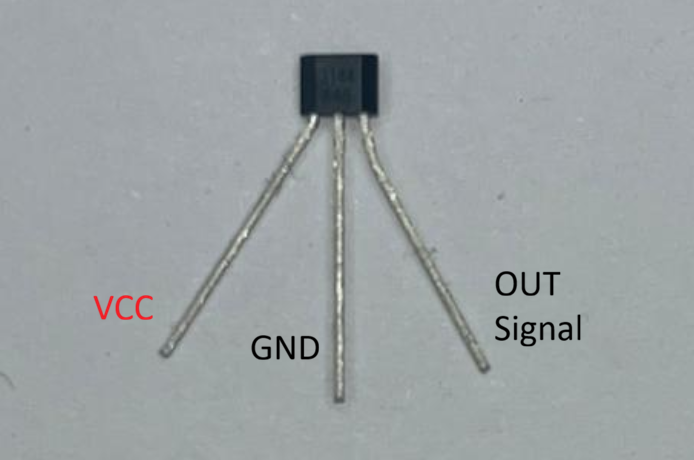
\includegraphics[width=\textwidth]{figures/nahaufnahme_a3144}
		\caption{Nahaufnahme des A3144}
		\label{bild:nahaufnahme_a3144}
	\end{minipage}
	\hfill
	\begin{minipage}{0.45\textwidth}
		\centering
		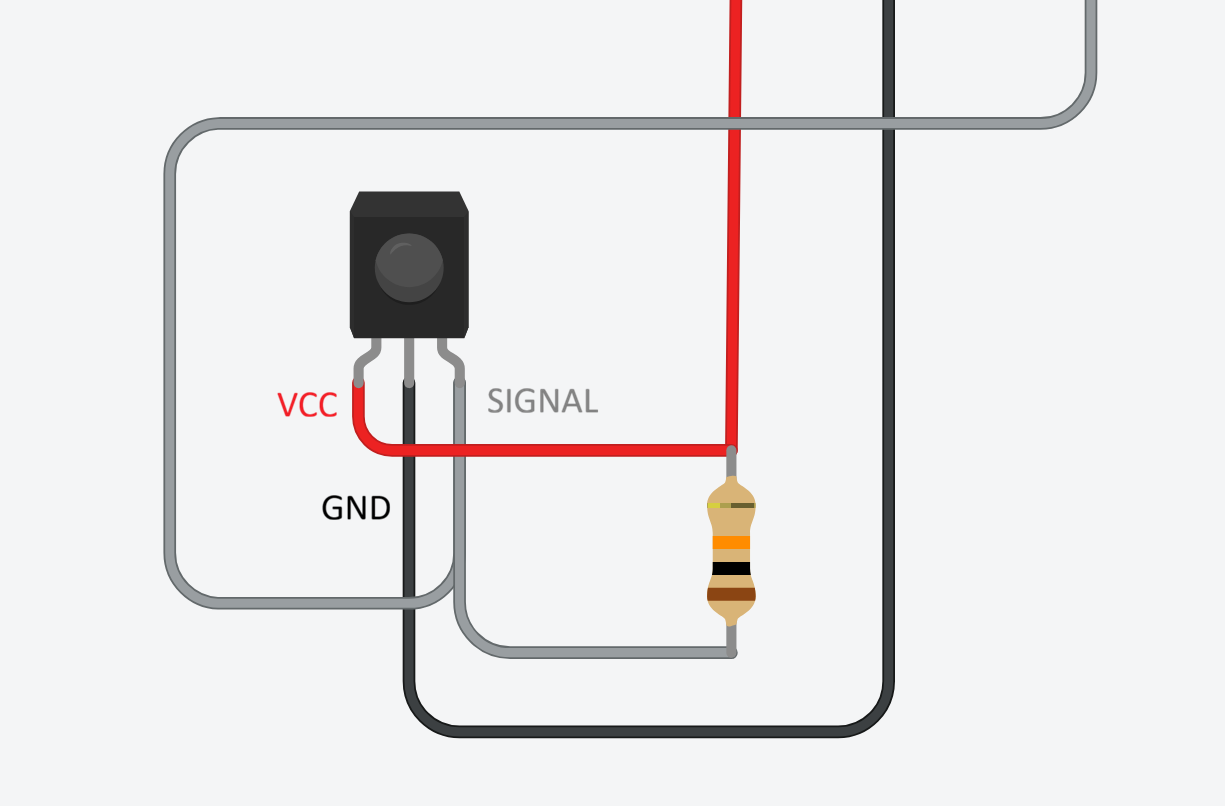
\includegraphics[width=\textwidth]{figures/Verschaltung}
		\caption{Verschaltung des A3144}
		\label{bild:verschaltung}
	\end{minipage}
	
\end{figure}

\subsubsection{Pull-Up Widerstandsberechnung}

Der A3144 besitzt einen Open-Collector-Ausgang, weshalb ein externer Pull-Up-Widerstand erforderlich ist, um im HIGH-Zustand eine definierte Ausgangsspannung zu erzeugen. Die Dimensionierung erfolgt auf Grundlage des Ohmschen Gesetzes. Der Widerstand bestimmt dabei den Strom im LOW-Zustand sowie die Schaltgeschwindigkeit des Signals. Die Berechnung erfolgt mit

\[
R_{PU} = \frac{V_{CC} - V_{CE(sat)}}{I_{LOW}}
\]

wobei \(V_{CC}\) die Versorgungsspannung, \(V_{CE(sat)}\) die Sättigungsspannung des Transistors (Datenblatt \(0{,}4\,V\)) und \(I_{LOW}\) der gewünschte Strom im eingeschalteten Zustand ist. Für \(V_{CC} = 3{,}3\,V\) und \(I_{LOW} = 1\,mA\) ergibt sich

\[
R_{PU} = \frac{3{,}3\,V - 0{,}4\,V}{0{,}001\,A} = 2{,}9\,k\Omega
\]

Als geeigneter Normwert wird \(3{,}3\,k\Omega\) gewählt. Ein kleinerer Widerstand erhöht den Strom und verbessert die Schaltgeschwindigkeit, während ein größerer Widerstand den Stromverbrauch reduziert, jedoch Slangsamere Signalflanken bringt.

Die Schaltgeschwindigkeit hängt vom Pull-Up-Widerstand ab, da dieser zusammen mit der parasitären Leitungskapazität \( C \) eine RC-Zeitkonstante bildet. Beim Übergang von LOW nach HIGH wird die Leitung über den Widerstand aufgeladen, wobei die Anstiegszeit durch die Zeitkonstante 

\[
\tau = R \cdot C
\]

bestimmt wird. Die Spannung steigt dabei exponentiell nach

\[
U(t) = U_{CC} \left(1 - e^{-\frac{t}{RC}} \right)
\]

an. Ein größerer Widerstand führt zu einer größeren Zeitkonstante \( \tau \) und somit zu einem langsameren Spannungsanstieg, während ein kleinerer Widerstand eine kleinere Zeitkonstante und damit eine schnellere Schaltflanke bewirkt.

\subsubsection{Schaltungsaufbau}

Um die korrekte Verdrahtung zu testen wurde von Diplomant Maximilian Koch ein Pyhton Programm geschrieben welches unter ``Bildverwis'' zu sehen ist. Der Output von diesem Programm ist unter ``Bildverweis'' zu sehen.

Aufbau auf einem Steckbrett zur Inbetriebnahme der Sensoren:

\begin{figure}[htbp]
    \centering
    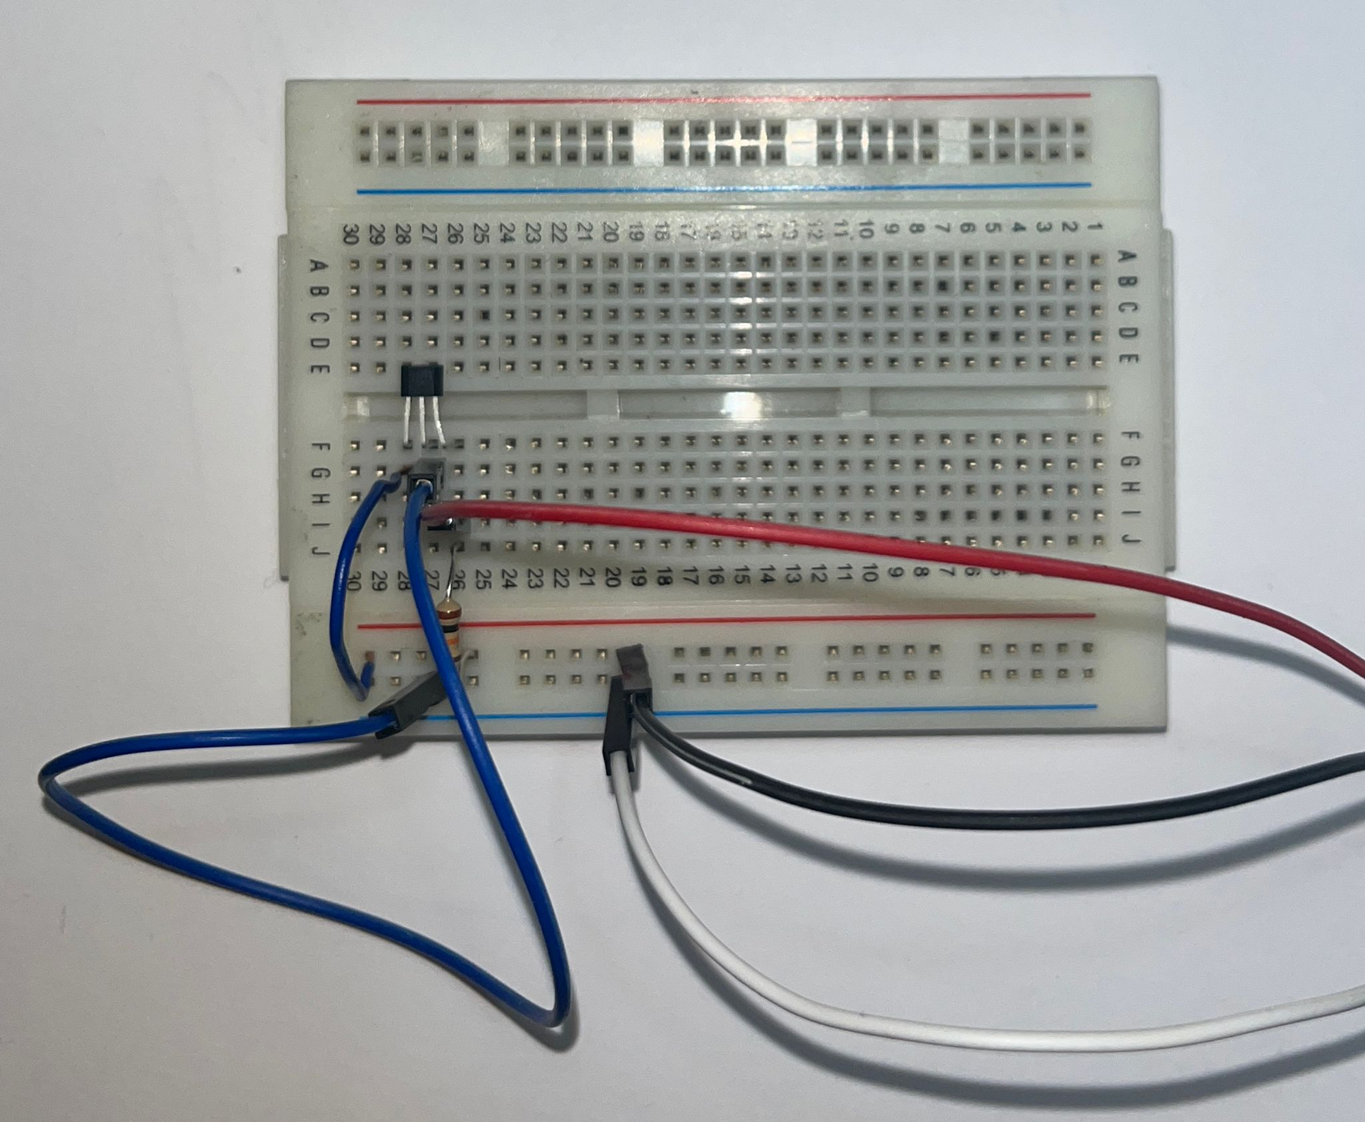
\includegraphics[width=0.7\textwidth]{figures/einzel.png}
    \caption{Einzelbeschaltung}
    \label{fig:einzel}
\end{figure}

rotes Jumper-Kabel 		-> Signal \newline
blaues Jumper Kabel mittig	-> GND \newline
blaues Jumper Kabel rechts	-> VCC \newline


\subsubsection{Matrix-entwicklung}
Wichtige Punkte zu beachten für die Matrix sind:
\begin{itemize}
	\item Leistungsaufnahme der Sensoren
	\item Schaltzeiten um Fehler zu verhindern
	\item Störsicherheit
\end{itemize}

\paragraph{Leistungsaufnahme}

Der gewählte A3144 Hall-Effekt Sensor benötigt typischerweise 4,4mA bis zu maximal 9 mA ``Quelle''. Bei acht parallel angeschlossenen Sensoren ergibt sich so ein Strombedarf von ca. 35 mA bis maximal 72 mA. Ein GPIO Pin des Raspberry Pi ist allerdings nur für ungefähr 16 mA fähig ``Quelle''. Deshalb wird für die Versorgung der Sensoren ein MOSFET als Schalter benötigt. \newline

\paragraph{Schaltzeiten}

Um für zuverlässige Auslesungen der Matrix zu sorgen müssen Anstiegs und Abfallzeiten der Signalleitungen als auch die Schaltzeiten der MOSFETS beachtet werden um überlappende Signale zu verhindern.
Dafür wird gesorgt indem Diplomant Maximilian Koch ein entsprechendes Delay im Code zur Auslesung der Matrix implementiert. \newline

\paragraph{Störsicherheit}

Die Matrix sollte so konzipiert und umgesetzt werden, dass zum einen keine Fehlerhaften Signale auf den Leitungen vorkommen. Diese Fälle wurden schon in den Punkten ``Querverweis'' und ``Querverweis'' gelöst, sodass diese nicht auftreten. Zum Schutz der GPIO Pins sind noch Gatewiderstände notwendig. Diese variieren je nach Gatekapazität von MOSFET zu MOSFET. Um das Gate auf LOW zu halten, wenn der GPIO PIN noch kein Signal sendet wurde auch am Gate des Mosfets ein 100kOhm Gate-Pulldown Widerstand eingebaut. Zuätzlich sollte die Matrix aber auch so umgesetzt werden, dass der Spieler auf dem Brett die Figuren bewegen kann, ohne darauf achten zu müssen, große Bewegungen um Felder zu machen, welche er nicht bespielen will.  

\vfill
\newpage

\subsubsection{Prototypenaufbau}

Bei der Erstellung des Prototypen in Form einer 2x2 Matrix wurden als MOSFETs 2 IRLZ44 N-Kanal verwendet, da diese bereits zur Verfügung standen. Diese sind jedoch nicht perfekt da bei einer Gate-Spannung von 3,3V Der $R_{\mathrm{DSon}}$ noch nicht minimal klein ist ``Quelle'', allerdings ist es für die Testung ausreichend und durch die geringe Last von maximal ca. 30mW ist Wärmeentstehung durch den Widerstand auch nicht problematisch.


\begin{table}[h]
\centering
\begin{tabular}{|l|c|l|}
\hline
\textbf{Bauteil} & \textbf{Anzahl} & \textbf{Bemerkung} \\ \hline
A3144 Hall-Sensor & 4 & Digitale Hall-Effekt Sensoren \\ \hline
IRLZ44N MOSFET & 2 & N-Kanal Logic-Level MOSFET \\ \hline
Gate-Pulldown Widerstand & 2 & 100 k$\Omega$ \\ \hline
Gate-Widerstand & 2 & 220 $\Omega$ \\ \hline
Pull-Up Widerstand & 2 & 4,7 k$\Omega$ \\ \hline
\end{tabular}
\caption{Verwendete elektronische Bauteile}
\label{tab:bauteile}
\end{table}

\begin{figure}[H]
\centering
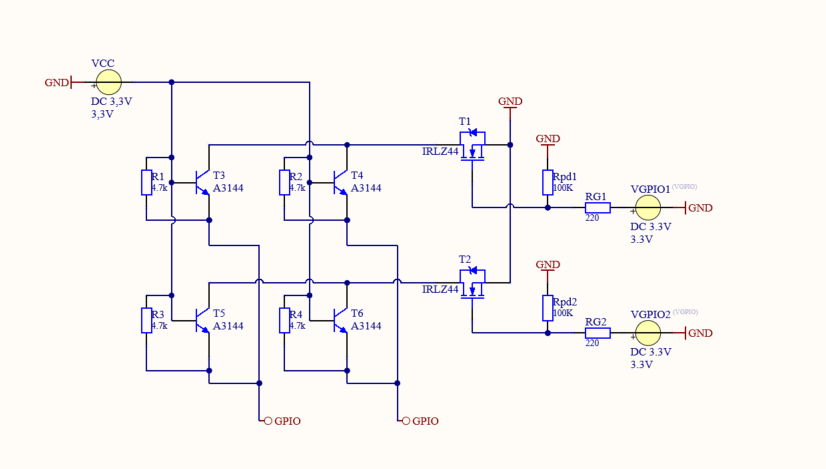
\includegraphics[width=1\textwidth]{figures/2x2Wiringplan.png}
\caption{2x2 Wiring Plan}
\label{fig:wiringplan}
\end{figure}

\begin{figure}[H]
\centering

\begin{minipage}{0.45\textwidth}
    \centering
    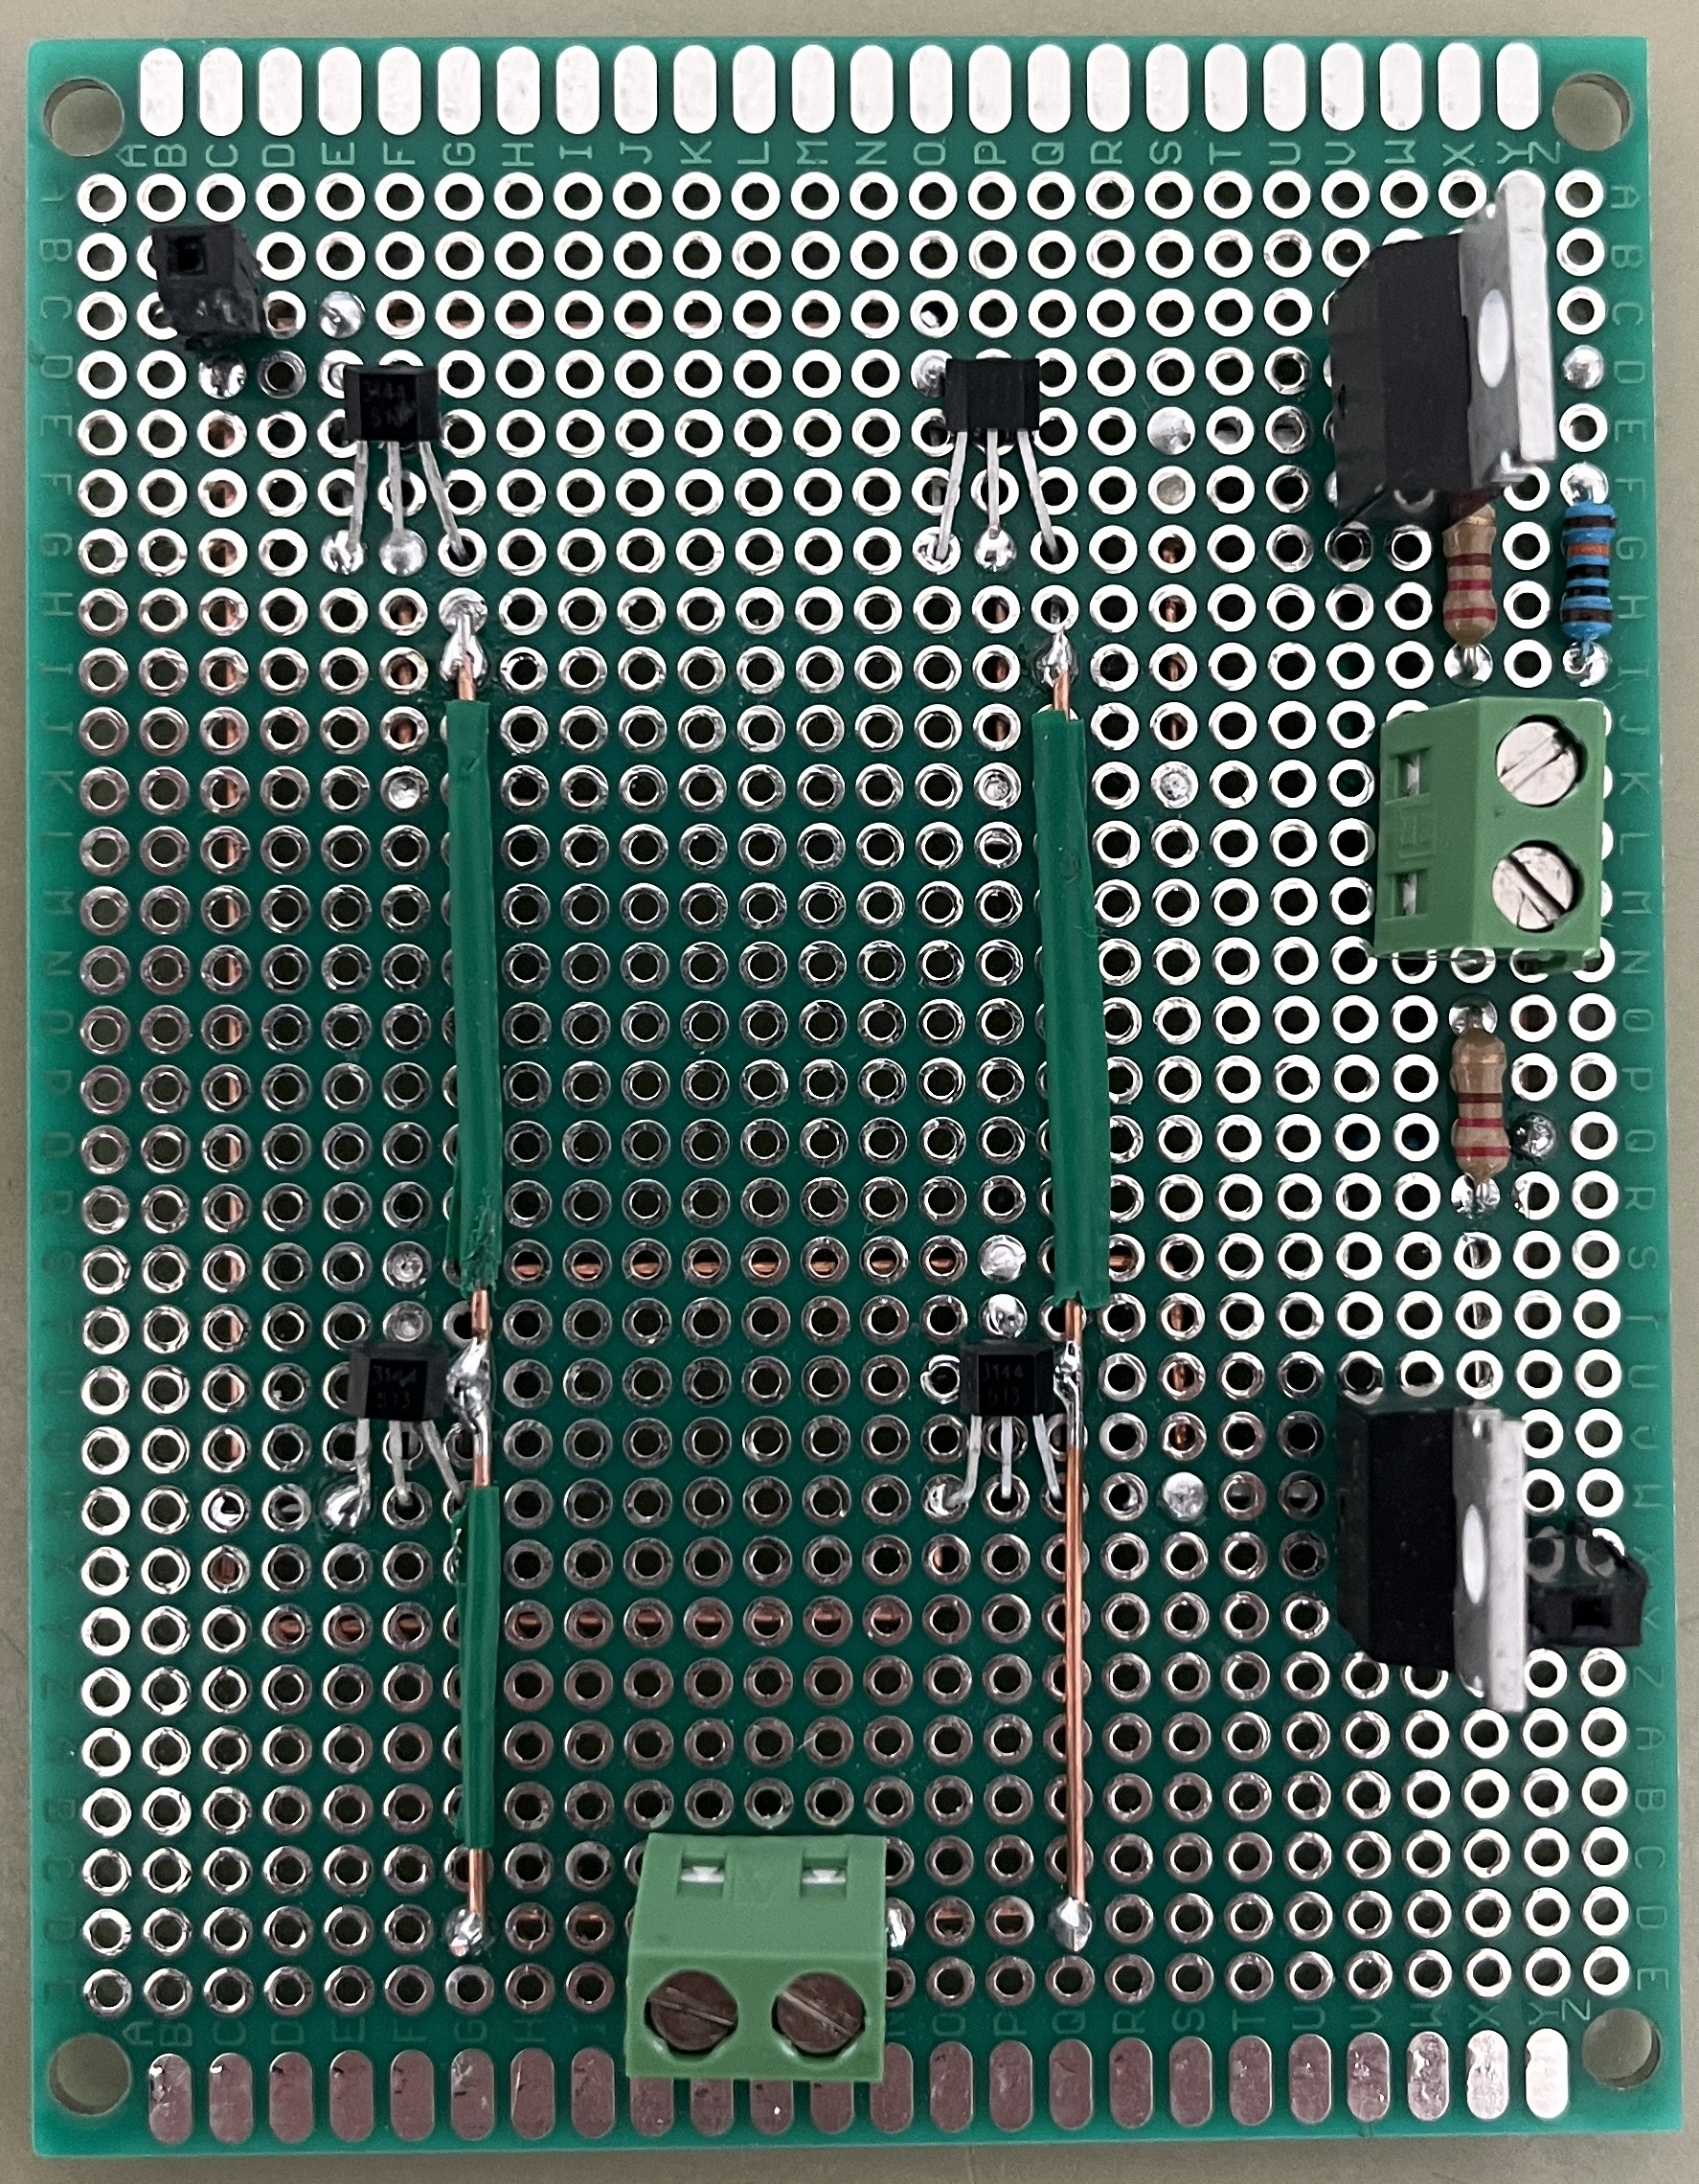
\includegraphics[width=7cm]{figures/PlatinenPrototyp2.jpg}
    \caption{Schaltplan der aufgebauten Schaltung}
    \label{fig:schaltplan}
\end{minipage}
\hfill
\begin{minipage}{0.5\textwidth}
\begin{itemize}
	\item Steckanschluss oben links		\newline-> 3,3V Spannungsversorgung
	\item Steckanschluss unten rechts	\newline-> Ground
	\item Blockklemme rechts			\newline-> GPIO Ausgänge Raspberry Pi
	\item Blockklemme unten			\newline-> GPIO Eingänge Raspberry Pi
	\newline
	
	Die Schaltung wurde als LOW-Side Beschaltung aufgebaut, das bedeuet, dass nicht mehr 3,3V aktiv durchgeschaltet werden, sondern der 			MOSFET den Ground durchschaltet
\end{itemize}
\end{minipage}
\end{figure}

Das Programm welches Diplomant Maximilian Koch geschrieben hat, um die Platine erfolgreich in Betrieb zu nehmen, ist unter Punkt ``Querverweis'' zu finden. 
\newpage


\subsection{Platinendesign}

Die Entwicklung des Schaltplans sowie das Layout der Leiterplatte wurden mit der Software Altium Designer in der Version 22.7.1 erstellt. Auf Basis der erstellten Konstruktionsdatein erfolgte die Fertigung der Leiterplatte durch den Leiterplattenhersteller JLCPCB. 

\begin{figure}[H]
\centering
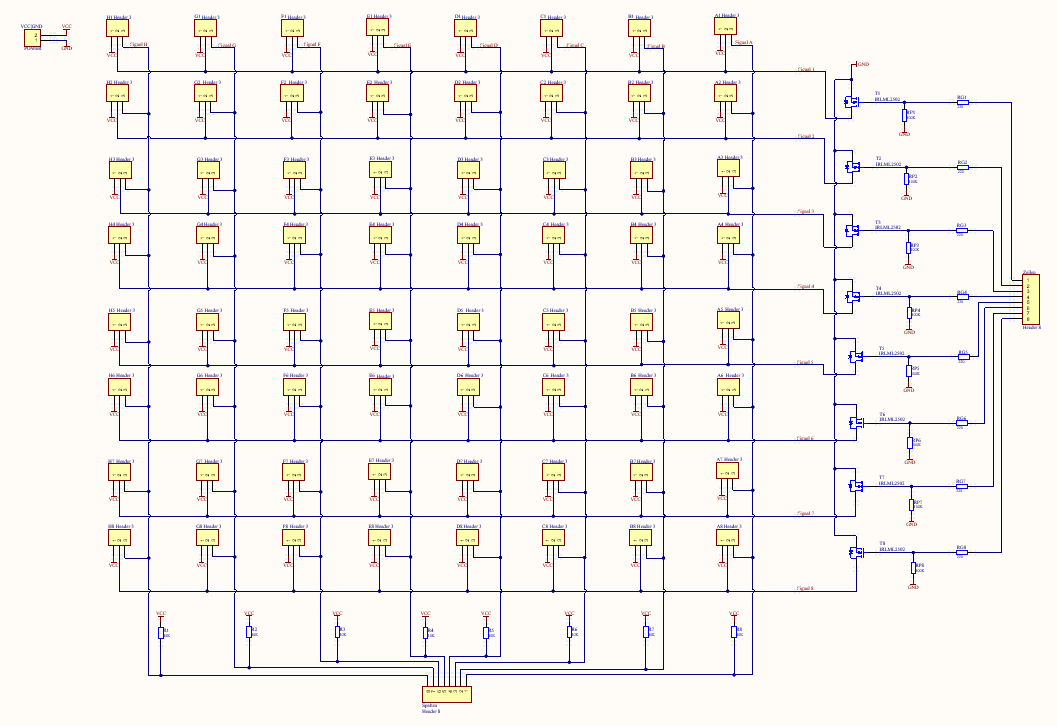
\includegraphics[width=1\textwidth]{figures/8x8Matrix.png}
\caption{8x8 LED-Matrix}
\label{fig:8x8matrix}
\end{figure}

Der Schaltplan ist so aufgebaut, dass rechts die Ausgänge vom Raspberry Pi sind welche die Zeilen aktiv ein und ausschalten. Unten sind die Anschlüsse für die Raspberry Pi Eingänge welche an den Signalleitungen der A3144 Sensoren hängen. 


\subsubsection{Altium Platinendesign}

Von diesem Schaltplan wurde nun ein 4-Lagiges PCB erstellt welches die Konstruktionsdatei für JLCPCB bereitstellen soll. Wichtig ist, dass die Felder und Anschlüsse so platziert werden wie diese berechnet wurden damit die Platine anschließend ins Gehäuse passt. 

Das Schachbrett besteht aus jeweils 64 Quadraten mit einer Seitenlänge von jeweils $28\,\mathrm{mm}$. Zwischen jeweils zwei benachbarten Feldern liegt ein Abstand von $2\,\mathrm{mm}$, sodass pro Reihe $7$ Zwischenräume entstehen. Die Gesamtlänge einer Seite berechnet sich daher aus $8 \cdot 28\,\mathrm{mm} + 7 \cdot 2\,\mathrm{mm} = 238\,\mathrm{mm}$. Da das Schachbrett quadratisch ist, beträgt auch die andere Seitenlänge $238\,\mathrm{mm}$. Wichtig noch zu beachten ist, dass der erste Sensor  $14\,\mathrm{mm}$ vom Rand entfernt platziert werden muss.

\begin{figure}[H]
    \centering
    % Hier wird das Bild aus dem Ordner "figures" geladen
    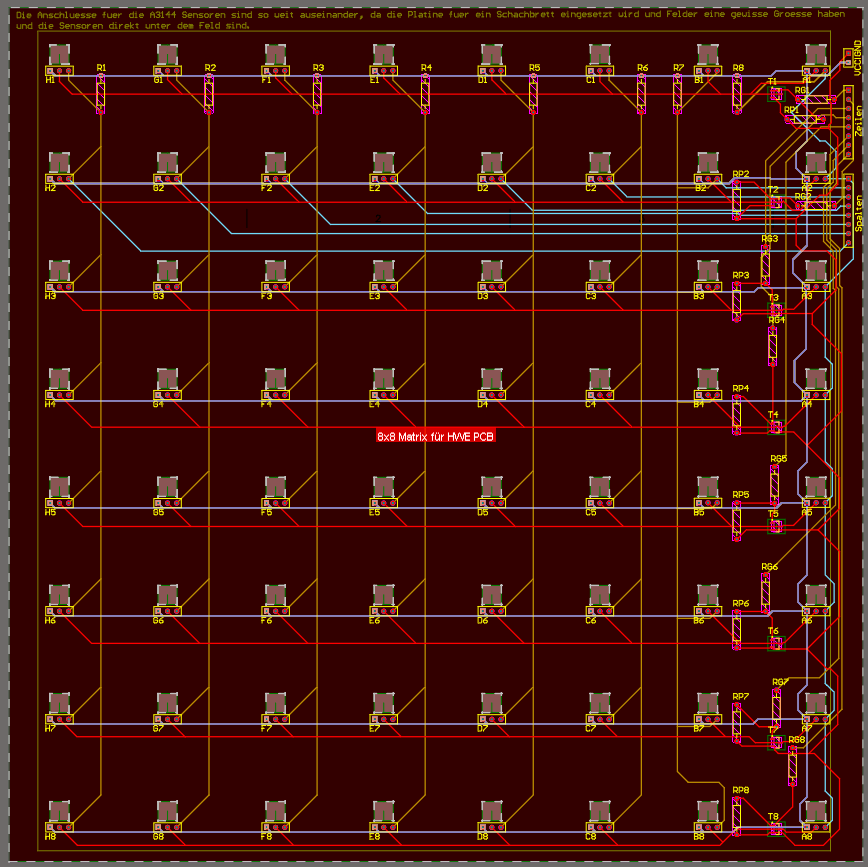
\includegraphics[width=0.72\textwidth]{figures/AltiumPCB.png}
    
    \caption{Geroutete Platine bereit für die Fertigung}
    \label{fig:altium_pcb}
\end{figure}

Um diese Platine Final zu bestellen wurde ein Finaler Designrulecheck für ein 4-lagiges JLC PCB gemacht (Designrules ``Quelle'') und erfolgreich mit null Errors durchgeführt und somit war die Platinenerstellung erledigt. 

\begin{figure}[H]
    \centering
    % Hier wird das JPEG-Bild geladen
    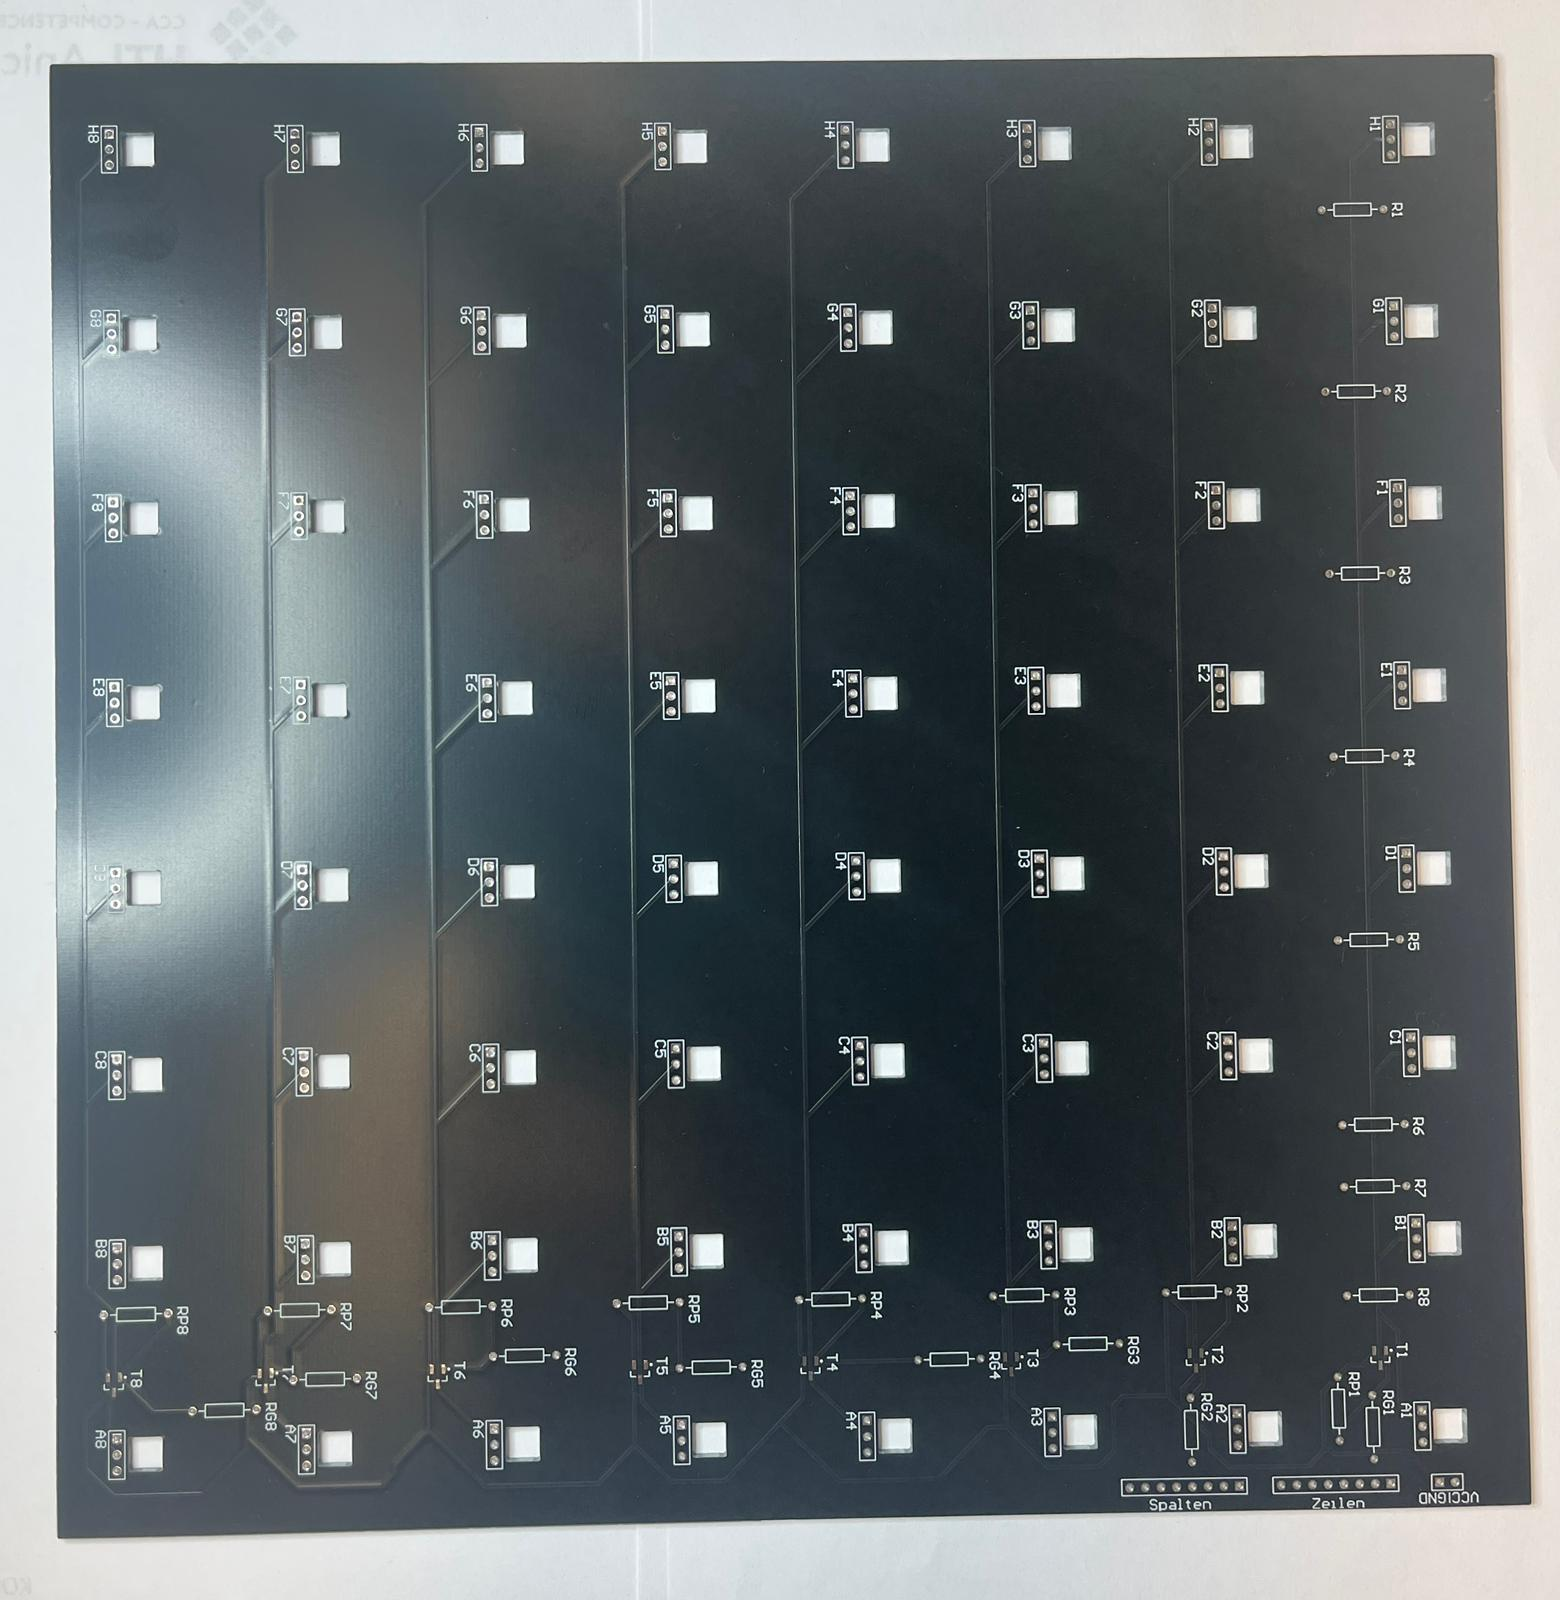
\includegraphics[width=0.8\textwidth, angle=90]{figures/JLCPCBPlatine.jpg}
    
    \caption{Unbestückte Platine}
    \label{fig:jlcpcb_platine}
\end{figure}

Die Platine wurde aus Kostengründen unbestückt bestellt und selbst bestückt. 

\subsection{Gehäusefertigung}

\subsection{Stromversorgung}